\documentclass[letterpaper]{article}
\usepackage[utf8]{inputenc}
\usepackage[parfill]{parskip}    % Activate to begin paragraphs with an empty line rather than an indent
\usepackage{graphicx}
\usepackage{amssymb}
\usepackage{amsmath}
\usepackage{amsthm}

\usepackage{afterpage}

\usepackage{algorithm}
\usepackage{algpseudocode}

\usepackage{verse}

\newtheorem{theorem}{Theorem}[section]
\newtheorem{corollary}{Corollary}[theorem]
\newtheorem{lemma}[theorem]{Lemma}

\theoremstyle{remark}
\newtheorem*{remark}{Remark}

\usepackage{epstopdf}
\usepackage{circuitikz}
\usepackage[separate-uncertainty = true,multi-part-units=single]{siunitx}
\usepackage{booktabs}
\usepackage{enumitem}
\usepackage[toc,page]{appendix}
\usepackage{color}
\usepackage{pgfplots}
\usepackage{pgfplotstable}
\usepackage{caption}
\usepackage{subcaption}
\usepackage{url}
\usepackage{multirow}
\usepackage{makecell}
\usepackage[round]{natbib}   % omit 'round' option if you prefer square brackets
\usepackage{titling}
\usepackage{siunitx}

\usepackage{setspace}
% \doublespacing
\usepackage{float}


\pgfplotsset{compat=1.14}

%  Special math symbols
%       floor, ceiling, angled brackets
%-----------------------------------------------------------------------
\newcommand{\floor}[1]{\left\lfloor #1\right\rfloor}
\newcommand{\ceil}[1]{\left\lceil #1\right\rceil}
\newcommand{\etal}{\textit{et al.}}
\newcommand{\RE}{\mathbb{R}}        % real space
\newcommand{\ZZ}{\mathbb{Z}}        % integers
\newcommand{\NN}{\mathbb{N}}        % natural numbers
\newcommand{\eps}{{\varepsilon}}    % prettier epsilon
%-----------------------------------------------------------------------
%  Tighter lists
%-----------------------------------------------------------------------
\newenvironment{itemize*}% Tighter itemized list
  {\begin{itemize}%
    \setlength{\itemsep}{-0.5ex}%
    \setlength{\parsep}{0pt}}%
  {\end{itemize}}
\newenvironment{description*}% Tighter description list
  {\begin{description}%
    \setlength{\itemsep}{-0.5ex}%
    \setlength{\parsep}{0pt}}%
  {\end{description}}
\newenvironment{enumerate*}% Tighter enumerated list
  {\begin{enumerate}%
    \setlength{\itemsep}{-0.5ex}%
    \setlength{\parsep}{0pt}}%
  {\end{enumerate}}
%-----------------------------------------------------------------------
% Typing shortcuts
%-----------------------------------------------------------------------
\newcommand{\X}{\mathbb{X}}
\newcommand{\SG}{\mathbf{S}}
\newcommand{\GE}{\mathcal{G}}
\newcommand{\ST}{\,:\,}
\renewcommand{\tilde}[1]{\widetilde{#1}}
\newcommand{\diam}{\mathrm{diam}}
\newcommand{\sq}{\square}
\newcommand{\half}[1]{\frac{#1}{2}}
\newcommand{\inv}[1]{\frac{1}{#1}}
\newcommand{\alg}{\textsf{SplitReduce}}
\newcommand{\sz}[1]{\sigma_{#1}}
\newcommand{\LL}{\mathcal{L}}
\newcommand{\softOmega}{\widetilde{\Omega}} 
\newcommand{\softO}{\widetilde{O}}
\newcommand{\OO}{O^*}  %or \widetilde{O}?

\newcommand{\norm}[1]{\left\lVert#1\right\rVert}

\newcommand{\dx}{\mathrm{d}x}
\newcommand{\dy}{\mathrm{d}y}
\newcommand{\dz}{\mathrm{d}z}
\newcommand{\dt}{\mathrm{d}t}
\newcommand{\du}{\mathrm{d}u}
\newcommand{\dtheta}{\mathrm{d}\theta}
\newcommand{\dq}{\mathrm{d}q}
\newcommand{\diff}{\mathrm{d}}
\newcommand{\dV}{\mathrm{d}V}
\newcommand{\dL}{\mathrm{d}L}
\newcommand{\dA}{\mathrm{d}A}
\newcommand{\dH}{\mathrm{d}H}
\newcommand{\df}{\mathrm{d}f}
\newcommand{\dg}{\mathrm{d}g}
\newcommand{\dr}{\mathrm{d}r}
\newcommand{\dw}{\mathrm{d}w}
\newcommand{\dv}{\mathrm{d}v}

\newcommand*\len[1]{\overline{#1}}

\newcommand{\dd}{Decadent Dwight cookies }
\newcommand{\hh}{Heavenly Hearst cookies }

\newcommand\note[1]{\marginpar{\textcolor{red}{#1}}}
\newcommand*{\tageq}{\refstepcounter{equation}\tag{\theequation}}

\newcommand*{\equals}{=}

\usepackage{fancyhdr}

\pgfplotscreateplotcyclelist{grayscale}{
    thick,white!10!black,mark=x,mark options=solid, dashed\\%
    thick,white!20!black,mark=o,mark options=solid\\%
}

\newcommand{\mat}[1]{\ensuremath{\begin{bmatrix}#1\end{bmatrix}}}
\newcommand{\eqn}[1]{\begin{alignat*}{2}#1\end{alignat*}}
\newcommand{\p}[2]{\frac{\partial #1}{\partial #2}}
\newcommand*{\thus}{&\implies\quad&}

\newcommand{\answer}[1]{\framebox{$\displaystyle #1 $}}

 
\pagestyle{fancy}
\fancyhf{}
\rhead{Rahul Arya}
\lhead{EE 16B}
\cfoot{\thepage}

\title{Lecture 1 - Notes}
\author{Rahul Arya}
\date{January 2019}
\begin{document}

\maketitle

\section{Overview}
In EE16A, we focused on analog circuits, often performing mathematical operations. However, analog circuits suffer from a high degree of susceptibility to noise. Consider, for instance, an analog circuit adding two 64 bit integers. Even if the levels of noise were as low \SI{1}{\nano\volt}, our circuit would have to run with voltages of the order of
\[
    2^{64} \cdot (\SI{1}{\nano\volt}) = \SI{18}{\giga\volt},
\]
in order to handle the full range of the input, a clearly impractical value.

The use of \emph{digital circuits} allows us to mitigate the problem of noise quite considerably, by adopting a discrete / quantized interpretation of a continuous signal. At its most basic level, a signal $V$ in digital logic corresponds to two different logical values: $0$ or $1$. Signals very close to $0$ correspond to logical $0$, while signals very close to $1$ (or some other maximum value) correspond to logical $1$. The errors allowed before a signal is incorrectly interpreted are known as the \emph{noise margins}, as shown below:  
\begin{center}
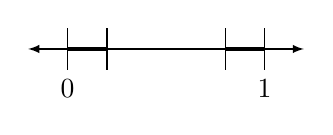
\begin{tikzpicture}[scale=2.5]
\draw[latex-latex] (-0.2,0) -- (1.2,0) ; %edit here for the axis
\foreach \x in  {0, 0.2, 0.8, 1} % edit here for the vertical lines
\draw[shift={(\x,0)},color=black] (0pt,3pt) -- (0pt,-3pt);
\foreach \x in {0, 1} % edit here for the numbers
\draw[shift={(\x,0)},color=black] (0pt,0pt) -- (0pt,-3pt) node[below] 
{$\x$};
\draw[very thick] (0, 0) -- (0.2, 0);
\draw[very thick] (0.8, 0) -- (1, 0);
\end{tikzpicture}
\end{center}

A key principle in digital logic is in avoiding the accumulation of noise across computations. Otherwise, even the most generous error bounds and the most noise-free computations will inevitably lead to error, as small errors accumulate over millions of computations. We wish to obtain a guarantee that if the inputs to our circuit lie within our noise margins, that the output signals will as well.

\section{CMOS}
To achieve this, we use what is known as CMOS logic (CMOS stands for ``complementary metal oxide semiconductors"). CMOS consists of two related components (hence ``complementary"): NMOS and PMOS. Both these components have the following function: they control a switch between two terminals, based on the signal supplied at a third terminal:
\begin{center}
\begin{circuitikz}[european] 
\draw(0, 0) node[left]{Control} to (0.8, 0);
\draw (1, 1) to[R] (1, -1);
\draw[-latex] (1.5, 0.6) -- (1.5, -0.6);
\end{circuitikz}
\end{center}

We call the control terminal the \emph{gate}, with the controlled current (as labelled) between the \emph{drain} and the \emph{source}.

Typically, in circuit diagrams, these components are drawn as follows, with $G$ representing the gate, $D$ representing the drain, and $S$ representing the source:

\begin{figure}[H]
\centering
\begin{subfigure}{.5\textwidth}
\centering
\begin{circuitikz}[american] 
\draw (0, 0) node[nmos] (nmos) {};
\draw (nmos.G) node[left]{$G$};
\draw (nmos.S) node[left]{$S$};
\draw (nmos.D) node[left]{$D$};
\end{circuitikz}
\caption{NMOS}
\end{subfigure}%
\begin{subfigure}{.5\textwidth}
\centering
\begin{circuitikz}[american] 
\draw (0, 0) node[pmos] (nmos) {};
\draw (nmos.G) node[left]{$G$};
\draw (nmos.S) node[left]{$S$};
\draw (nmos.D) node[left]{$D$};
\end{circuitikz}
\caption{PMOS}
\end{subfigure}
\end{figure}

Of course, voltages are only meaningful when measured between two points. Both NMOS and PMOS devices respond to the voltage between the gate and the source, denoted as $V_{GS}$. However, from the diagram above, the drain and the source appear to be symmetrical, so it is not apparent which terminal is which. For NMOS devices, the source terminal is the terminal at a lower voltage, while for PMOS devices, the source terminal is the terminal at a higher voltage.

Now, we will discuss the precise behavior of these components in more detail. For NMOS devices, a voltage $V_{GS}$ that is near $0$ (more precisely, when $V_{GS} < V_{th, N}$ for some threshold voltage $V_{th, N}$) will cause current to be blocked between the drain and the source, while a voltage $V_{GS}$ that is near some peak voltage $V_{dd}$ ($V_{GS} > V_{th, P}$) will allow current to flow. 

This behavior is summarized in the below figures, modelling NMOS and PMOS devices using switches:

\begin{figure}[H]
\centering
\begin{subfigure}{.5\textwidth}
\centering
\begin{circuitikz}[american] 
\draw (0, 0) node[ocirc]{} node[above]{$G$};
\draw (1, -1) node[ocirc]{} node[below]{$S$} to[nos] (1, 1) node[ocirc]{} node[above]{$D$};
\draw (0, 0) to[open, v=$V_{GS}$] (1, -1);
\end{circuitikz}
\caption{$V_{GS} < V_{th, N}$}
\end{subfigure}%
\begin{subfigure}{.5\textwidth}
\centering
\begin{circuitikz}[american] 
\draw (0, 0) node[ocirc]{} node[above]{$G$};
\draw (1, -1) node[ocirc]{} node[below]{$S$} to[ncs] (1, 1) node[ocirc]{} node[above]{$D$};
\draw (0, 0) to[open, v=$V_{GS}$] (1, -1);
\end{circuitikz}
\caption{$V_{GS} > V_{th, N}$}
\end{subfigure}
\captionsetup{labelformat=empty}
\caption{The behavior of an NMOS device.}
\end{figure}

\begin{figure}[H]
\centering
\begin{subfigure}{.5\textwidth}
\centering
\begin{circuitikz}[american] 
\draw (0, 0) node[ocirc]{} node[above]{$G$};
\draw (1, -1) node[ocirc]{} node[below]{$S$} to[ncs] (1, 1) node[ocirc]{} node[above]{$D$};
\draw (0, 0) to[open, v=$V_{GS}$] (1, -1);
\end{circuitikz}
\caption{$V_{GS} < V_{th, P}$}
\end{subfigure}%
\begin{subfigure}{.5\textwidth}
\centering
\begin{circuitikz}[american] 
\draw (0, 0) node[ocirc]{} node[above]{$G$};
\draw (1, -1) node[ocirc]{} node[below]{$S$} to[nos] (1, 1) node[ocirc]{} node[above]{$D$};
\draw (0, 0) to[open, v=$V_{GS}$] (1, -1);
\end{circuitikz}
\caption{$V_{GS} > V_{th, P}$}
\end{subfigure}
\captionsetup{labelformat=empty}
\caption{The behavior of a PMOS device.}
\end{figure}

\section{Simple Inverters}
Now, we will try to build circuits that do something interesting, using these new CMOS components. The first circuit we will build is an inverter - given a signal corresponding to a logical $0$, it will output a signal corresponding to logical $1$, and given a signal corresponding to a logical $1$, it will output a signal corresponding to logical $0$. We can represent the behavior of this circuit usign a truth table, as follows:
\begin{center}
  \begin{tabular}{ | l | r | }
    \hline
    IN & OUT \\ \hline
    0 & 1 \\ \hline
    1 & 0 \\
    \hline
  \end{tabular}
\end{center}

The following circuit is one possible implementation of an inverter, using a single NMOS device:
\begin{center}
\begin{circuitikz}[american] 
\draw (0, 0) node[nmos] (nmos) {};
\draw (nmos.G);
\draw (nmos.S);
\draw (nmos.D);
\draw(nmos.D) to[R, R=\SI{1}{\mega\ohm}] (0, 3) node[above]{$V_{dd}$};
\draw(nmos.S) to (0, -1) node[ground]{};
\draw(-1, 0) node[circ]{} node[left]{IN} to (nmos.G);
\draw (0, 1) to (1, 1) node[circ]{} node[right]{OUT};
\end{circuitikz}
\end{center}
Let's see why this circuit behaves like an inverter. To do so, we should consider the two possible logical values of the input: logical $0$, and logical $1$.

When the input is at logical $0$, the source and gate of the NMOS transistor are at equal voltages, so $V_{GS} < V_{th, N}$. Thus, the NMOS transistor's switch will open, so we obtain the following equivalent circuit:
\begin{center}
\begin{circuitikz}[american] 
\draw(0, 1) to[R, R=\SI{1}{\mega\ohm}] (0, 3) node[above]{$V_{dd}$};
\draw (0, -1) to (0, -1) node[ground]{};
\draw(-2, 0) node[circ]{} node[left]{IN} to (-1, 0);
\draw (0, 1) to (1, 1) node[circ]{} node[right]{OUT};
\draw (-1, 0) node[ocirc]{} node[above]{$G$};
\draw (0, -1) node[ocirc]{} node[left]{$S$} to[nos] (0, 1) node[ocirc]{} node[left]{$D$};
\end{circuitikz}
\end{center}
When no current is drawn from the output terminal, no voltage drops along the resistor, so the output terminal remains at $V_{dd}$, corresponding to a logical $1$, as we expect.

When the input is at logical $1$, the gate of the NMOS transistor will be at voltage $V_{dd} > V_{th, N}$. Thus the NMOS transistor's switch will close, so we obtain the following equivalent circuit: 
\begin{center}
\begin{circuitikz}[american] 
\draw(0, 1) to[R, R=\SI{1}{\mega\ohm}] (0, 3) node[above]{$V_{dd}$};
\draw (0, -1) to (0, -1) node[ground]{};
\draw(-2, 0) node[circ]{} node[left]{IN} to (-1, 0);
\draw (0, 1) to (1, 1) node[circ]{} node[right]{OUT};
\draw (-1, 0) node[ocirc]{} node[above]{$G$};
\draw (0, -1) node[ocirc]{} node[left]{$S$} to[ncs] (0, 1) node[ocirc]{} node[left]{$D$};
\end{circuitikz}
\end{center}

As can be seen, the output terminal is connected directly to ground, so the output of this circuit will be a logical $0$. Thus, its behavior matches its truth table for both possible inputs, so this circuit is an accurate model of an inverter.

Observe also that small levels of noise at the input do not affect the output signal at all, so this circuit does not allow noise to accumulate across chained circuits, as we had hoped.

\section{Efficient Inverters}
However, this inverter has a number of drawbacks. Most notably, observe that when the input is at logical $1$, current continually passes through the resistor. If we assume $V_{dd} = \SI{1}{\volt}$, a realistic value, then we find that the static power consumption of this transistor is
\[
    P = \frac{V^2}{R} = \SI{1}{\micro\watt}.
\]
This doesn't seem like very much. But when we consider that a modern electronic processor has upwards of $N = 10^9$ transistors, we find that this power consumption adds up to a total of
\[
    P_{device} = PN = \SI{1}{\kilo\watt},
\]
which is an unreasonably large quantity, especially for devices like smartphones or laptops.

It turns out that, by combining NMOS and PMOS devices, we can produce an inverter that has no static power consumption in either state. To do so, we need to first consider the opposite of the previous device, by building an inverter using a single PMOS device. We can do so as follows:
\begin{center}
\begin{circuitikz}[american] 
\draw (0, 2) node[pmos] (nmos) {};
\draw (nmos.G);
\draw (nmos.S);
\draw (nmos.D);
\draw(nmos.S) to (0, 3) node[above]{$V_{dd}$};
\draw(nmos.D) to[R, R=\SI{1}{\mega\ohm}] (0, -1) node[ground]{};
\draw(-1, 2) node[circ]{} node[left]{IN} to (nmos.G);
\draw (0, 1) to (1, 1) node[circ]{} node[right]{OUT};
\end{circuitikz}
\end{center}

The analysis of this circuit is extremely similar to that of the NMOS inverter. We again consider both possible logical states of the input signal, determine the position of the switch in our model of the transistor, and draw the equivalent circuits, as follows:

\begin{figure}[H]
\centering
\begin{subfigure}{.5\textwidth}
\centering
\begin{circuitikz}[american] 
\draw(0, 1) to[R, R=\SI{1}{\mega\ohm}] (0, -1) node[ground]{};
\draw (0, 1) to[ncs] (0, 3) node[above]{$V_{dd}$};
\draw(-2, 2) node[circ]{} node[left]{IN} to (-1, 2);
\draw (0, 1) node [ocirc] {} node[left] {$D$} to (1, 1) node[circ]{} node[right]{OUT};
\draw (-1, 2) node[ocirc]{} node[above]{$G$};
\draw (0, 3) node[ocirc]{} node[left]{$S$};
\end{circuitikz}
\caption{Input at logical $0$.}
\end{subfigure}%
\begin{subfigure}{.5\textwidth}
\centering
\begin{circuitikz}[american] 
\draw(0, 1) to[R, R=\SI{1}{\mega\ohm}] (0, -1) node[ground]{};
\draw (0, 1) to[nos] (0, 3) node[above]{$V_{dd}$};
\draw(-2, 2) node[circ]{} node[left]{IN} to (-1, 2);
\draw (0, 1) node [ocirc] {} node[left] {$D$} to (1, 1) node[circ]{} node[right]{OUT};
\draw (-1, 2) node[ocirc]{} node[above]{$G$};
\draw (0, 3) node[ocirc]{} node[left]{$S$};
\end{circuitikz}
\caption{Input at logical $1$.}
\end{subfigure}
\end{figure}

Here, we see that the output signal is again what we expect. However, when the input is at logical $1$, no power is consumed, whereas when the input is at logical $0$, there is some static power. Looking at our previous NMOS inverter, we see the opposite behavior, with power consumed when the input is at logical $1$ but not a logical $0$.

It turns out that, by combining these two circuits, we can generate a so-called CMOS inverter that combines the best aspects of both of these circuits, and removes the need for a \SI{1}{\mega\ohm} resistor. We can do so as follows:
\begin{center}
\begin{circuitikz}[american] 
\draw (0, 0) node[left]{IN} node[circ]{};
\draw (1, 1) node[pmos] (pmos) {};
\draw (pmos.S) to (1, 2) node[above]{$V_{dd}$};
\draw (0, 0) to (0, 1);
\draw (0, 0) to (0, -1);
\draw (1, -1) node[nmos] (nmos) {};
\draw (nmos.S) node[ground] {};
\draw (pmos.D) to (nmos.D);
\draw (1, 0) to (1.5, 0) node[circ]{} node[right] {OUT};
\end{circuitikz}
\end{center}

Let's see why this works. As before, we have to consider two cases: the input signal of logical $0$, and logical $1$. Applying our understanding of the behavior of NMOS and PMOS devices as modeled as switches, we obtain the following two equivalent circuits in these two cases:

\begin{figure}[H]
\centering
\begin{subfigure}{.5\textwidth}
\centering
\begin{circuitikz}[american] 
\draw(0, 1) to[nos] (0, -1) node[ground]{};
\draw (0, 1) to[ncs] (0, 3) node[above]{$V_{dd}$};
\draw(-2, 1) node[circ]{} node[left]{IN};
\draw (-2, 1) to (-2, 2) to (-1, 2) node[ocirc] {};
\draw (-2, 1) to (-2, 0) to (-1, 0) node[ocirc] {};
\draw (0, 1) to (1, 1) node[circ] {} node[right] {OUT};
\end{circuitikz}
\caption{Input at logical $0$.}
\end{subfigure}%
\begin{subfigure}{.5\textwidth}
\centering
\begin{circuitikz}[american] 
\draw(0, 1) to[ncs] (0, -1) node[ground]{};
\draw (0, 1) to[nos] (0, 3) node[above]{$V_{dd}$};
\draw(-2, 1) node[circ]{} node[left]{IN};
\draw (-2, 1) to (-2, 2) to (-1, 2) node[ocirc] {};
\draw (-2, 1) to (-2, 0) to (-1, 0) node[ocirc] {};
\draw (0, 1) to (1, 1) node[circ] {} node[right] {OUT};
\end{circuitikz}
\caption{Input at logical $1$.}
\end{subfigure}
\end{figure}

\section{NAND and NOR gates}
Thus, we clearly see that this new CMOS inverter behaves as we would expect, with the output signal always the logical opposite of the logical value of the input signal, and unaffected by any small levels of noise in the input signal. In addition, however, notice, when no load is connected to the output terminal, that no static power is drawn in either case, making this new inverter superior to either of the two we previously considered.

Now, we will consider some more complex gates - specifically, the NAND and NOR gates. These gates take two inputs, not one, but still produce a single output. The truth table of NOR is outlined below:
\begin{center}
  \begin{tabular}{ | l | c | r | }
    \hline
    A & B & NOR(A, B) \\ \hline
    0 & 0 & 1 \\ \hline
    1 & 0 & 0 \\ \hline
    0 & 1 & 0 \\ \hline
    1 & 1 & 0 \\ \hline
  \end{tabular}
\end{center}

Essentially, this gate produces an output of logical $1$ only when both of the inputs are $0$, and outputs logical $0$ in all other cases.

What is important about the NAND and NOR gates is that they are \emph{universal} gates. This means that all other boolean functions can be implemented by creating a circuit consisting solely of that one type of gate. This is very useful, since it means that if we know how to produce NAND or NOR gates using whatever components we have, then we know how to use these components to produce any other digital function.

To produce a NOR gate (or any other boolean function) using CMOS, we typically divide the problem into two parts: ``pull-up" and ``pull-down". The pull-down portion of a gate consists of those components that force the output to be logical $0$, and the pull-up portion consists of those that force the output to be logical $1$. For any possible input, we want exactly one of the pull-up and pull-down portions to be active - if both are active, then we may short our power rails, while if neither are active, then our output may be disconnected entirely.

In the CMOS inverter we constructed previously, the single NMOS transistor connected to ground formed the pull-down portion of the circuit, and the single PMOS transistor connected to $V_{dd}$ formed the pull-up portion of the circuit. In general, we always use NMOS transistors to pull the output down, and always use PMOS transistors to pull it up.

Thus, we can draw an arbitrary digital circuit modelling a single gate as follows:
\begin{center}
\begin{circuitikz}[american] 
    \draw (0, 2) node[draw,minimum width=2cm,minimum height=1cm] {pull-up};
    \draw (0, 0) node[draw,minimum width=2cm,minimum height=1cm] {pull-down};
    \draw (0, 1) to (2, 1) node[circ]{} node[right]{OUT};
    \draw (0, 1.5) to (0, 0.5);
    \draw (0, 2.5) to (0, 3) node[above] {$V_{dd}$};
    \draw (0, -0.5) node[ground] {};
\end{circuitikz}
\end{center}

Now, let's try constructing the pull-down portion of our NOR gate. The NOR gate should be pulled down to logical zero whenever either input signal is logical $1$. Thus, we should place two NMOS transistors in parallel linking the output to ground, with each transistor corresponding to one of the input signals, so that if either signal is $1$, then its corresponding transistor will pull the OUTPUT to ground.

We now have a circuit that looks like this:
\begin{center}
\begin{circuitikz}[american] 
    \draw (0, 1) node[draw,minimum width=2cm,minimum height=1cm] {pull-up};
    \draw (0, 0.13) to (2, 0.13) node[circ]{} node[right]{OUT};
    \draw (0, 1.5) to (0, 2) node[above] {$V_{dd}$};
    \draw (-0.5, -1) node[nmos] (nmos1) {};
    \draw (0.5, -1) node[nmos, xscale=-1] (nmos2) {};
    \draw (nmos2.D) to (nmos1.D);
    \draw (nmos2.S) to (nmos1.S);
    \draw (nmos1.G) node[circ] {} node[left] {$A$};
    \draw (nmos2.G) node[circ] {} node[right] {$B$};
    \draw (0, -1.76) node[ground] {};
    \draw (0, 0.5) to (0, -0.24);
\end{circuitikz}
\end{center}

Now, when either $A$ or $B$ is logical $1$, the output signal is pulled down to logical $0$. However, when both $A$ and $B$ are set to logical $0$, the switches in both transistors open, and the output node is left floating. To address this, we will now aim to construct a pull-up network that acts exactly in this case. 

Incidentally, it can be shown (and will be shown in CS 61C) that any pull-down network has a corresponding pull-up network that ensures that the voltage sources are never shorted to ground, and that the output node is never disconnected from both rails. However, we do not need this proof for this specific example.

Our pull-up network requires both $A$ and $B$ to be set to logical $0$, for a connection to be made between $V_{dd}$ and the output. Clearly, we should place two PMOS transistors in series, connecting one transistor to each input signal. Thus, only when both signals are logical $0$ will the switches for both transistors close, and a connection made to the output. Constructing this circuit, we obtain:
\begin{center}
\begin{circuitikz}[american] 
    \draw (0, 0.13) to (2, 0.13) node[circ]{} node[right]{OUT};
    \draw (-0.5, -1) node[nmos] (nmos1) {};
    \draw (0.5, -1) node[nmos, xscale=-1] (nmos2) {};
    \draw (nmos2.D) to (nmos1.D);
    \draw (nmos2.S) to (nmos1.S);
    \draw (nmos1.G) node[circ] {} node[left] {$A$};
    \draw (nmos2.G) node[circ] {} node[right] {$B$};
    \draw (0, -1.76) node[ground] {};
    \draw (0, 1) node[pmos] (pmos1) {};
    \draw (0, 2.5) node[pmos] (pmos2) {};
    \draw (pmos1.D) to (0, -0.24);
    \draw (pmos1.S) to (pmos2.D);
    \draw (pmos2.S) to (0, 3.5) node[above] {$V_{dd}$};
    \draw (pmos2.G) node[circ] {} node[left] {$A$};
    \draw (pmos1.G) node[circ] {} node[left] {$B$};
\end{circuitikz}
\end{center}

Similar techniques may be used to construct a NAND gate.

\end{document}
